%This is chapter 4
%%=========================================
\chapter{Result}

Brief assessment of the overall goals (or recap?) What to be discussed in this chapter...
This section presents a walk through of the results...

\section{three-voxel-loader}
Include picture of voxelized chicken here
\subsection{Level Of Detail}
Include picture of torus with low LOD
\subsection{Performance}
Not optimized, a lot of unnecessary voxel geometry rendered when only outer mesh is visible.
\subsection{Loading support}
- XML
- VOX
- BINVOX -> Separate repo!
- 3D array

\subsection{Example}
An example is available on GitHub pages (repo)

\section{Voxelizer}
General overview of the engine.... Completely redesigned.. Features: Extendible ...
\subsection{Voxelization}

side by side image of anvil and the anvil voxelized.

As you can see from the figure xxx, the system support coloring.....
\begin{figure}[h]
    \centering
    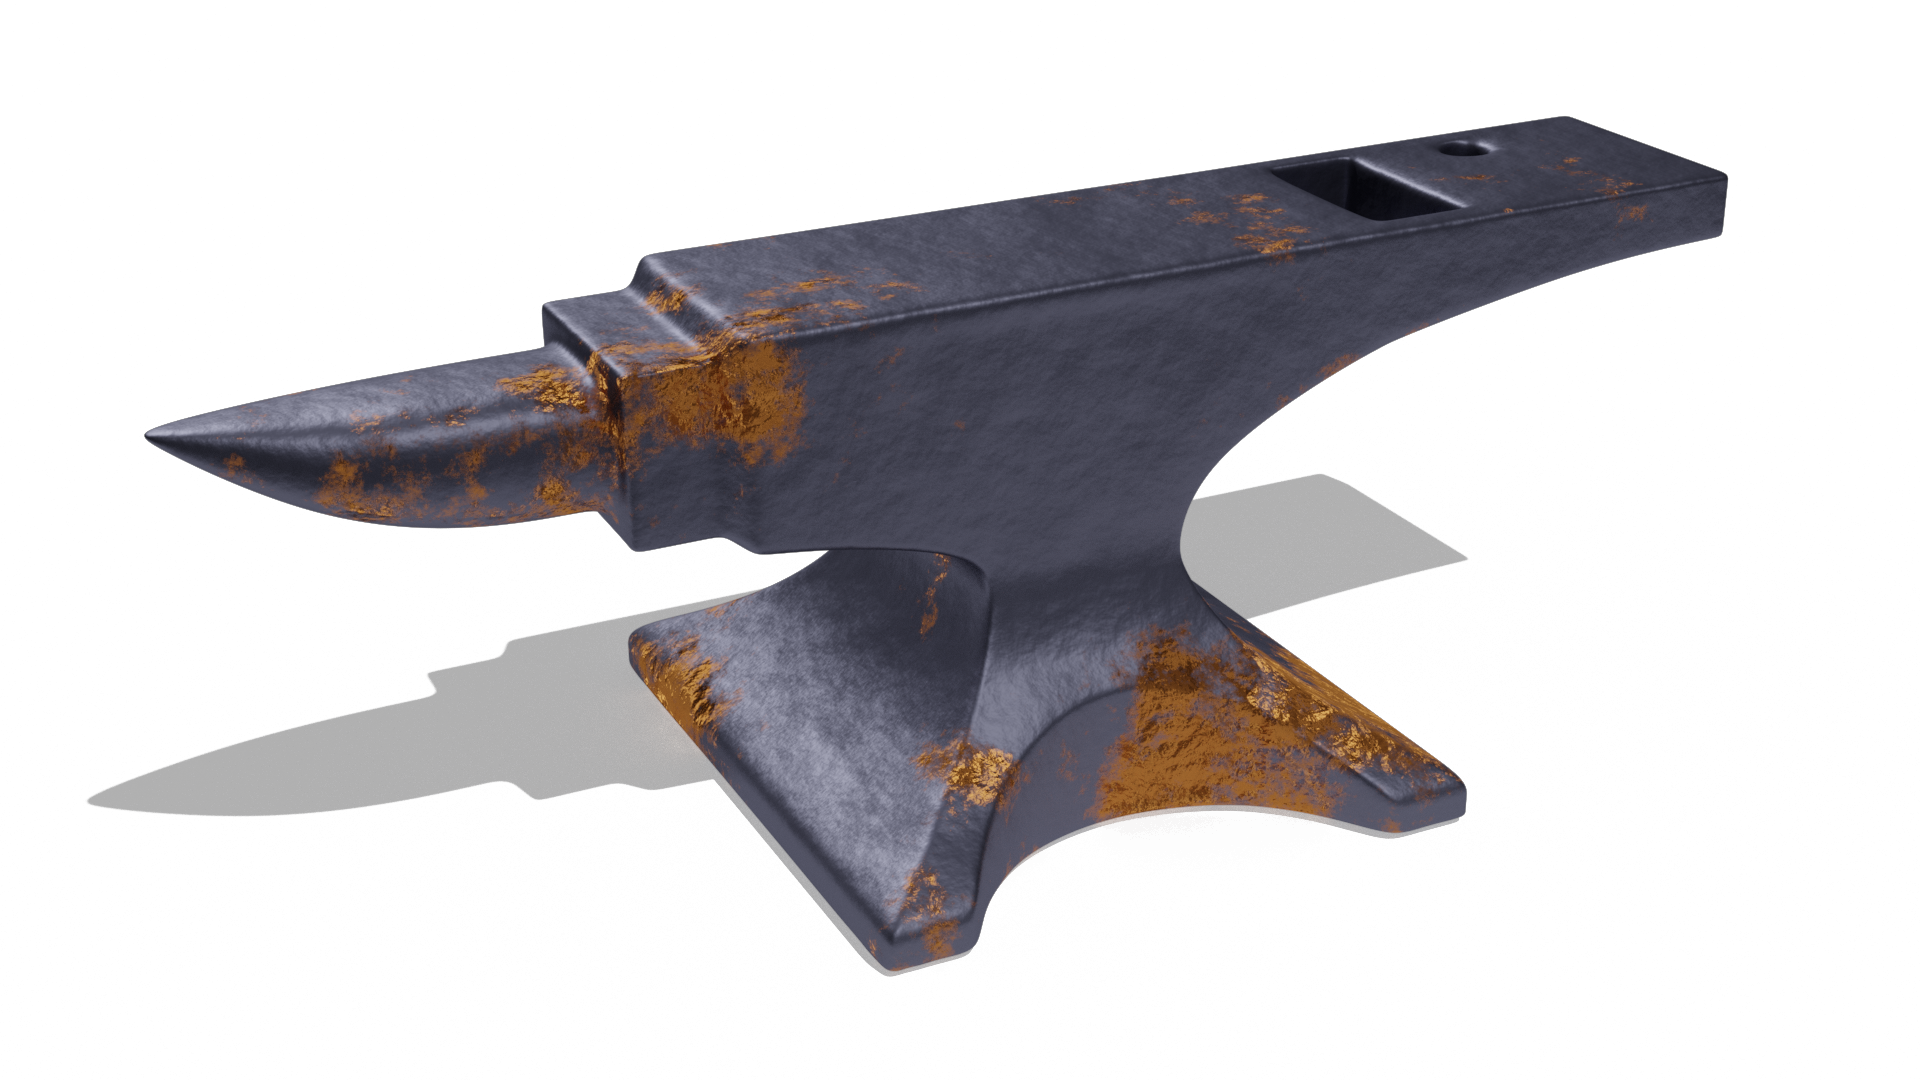
\includegraphics[width=\textwidth]{sections/result/figures/anvil-render.png}
    \caption{Render of anvil 3D model.}
    \label{fig:anvil-render}
\end{figure}

\subsection{Visual inspection}
No holes, accurate representation
Compare to requirement specification.

\subsection{Performance}
Do some tests and present them in a table.
Compare to requirement specification acceptance criteria.

\subsection{Importing}
This will be left up to the user. Supports all three.js meshes....

\subsection{Exporting}
Several formats...
- XML
- BINVOX
- 3D array
- ndarray

\subsection{Usage example}
Example of how to use the library with code!!!! HERE!!!!
\lstinputlisting[language=JavaScript,style=numbers]{sections/methodology/code/voxelizer.js}

\section{Voxelizer Desktop}
TODO
Cross compatibility
Speed
Simple to use
Secure

\section{JSDoc Action}
Easy automation of JSDoc generation and publication.
Included in MAIN JSDOC REPO!!! 10.000 stars and 38.000 users!!!

Supports templates and all that JSDoc3 natively supports.
Can use other actions to deploy docs to arbitrary service.


\section{Supportive projets}
\subsection{BINVOX}
JS module
Binary format...
Parses BINVOX files into JSON.
Builds BINVOX from JSON.
Works according to the official specification
Cross platform support (Node.js and Browser), ES6 and UMD. 

\subsection{file-existence-action}
Simple GitHub action to check for the existence of files.

\subsection{file-reader-action}
Simple GitHub action to read the contents of a file.

\section{Automation}
More or less fully automated all build and release/publishing steps.
\subsection{JavaScript modules}
- Building
- Testing
- coverage upload to coveralls
- Security analysis with LGTM
- JavaScript documentation Generation and deployment of the docs to GH pages.
- Publishing module to NPM.

\subsection{GitHub Actions}
- automation of "node-modules" installation setup
- automatic update of major version tags according to guidelines recommended by GitHub.

\subsection{LaTeX automation?}
Should i include this?

\section{Open-source community}
Several of the projects has already gained interest by the public.
Promotion og JSDoc Action in the main repo with 38 thousand users.

\subsection{Statistics}
Number of stars, weekly downloads, etc
\subsection{Feedback}
Several filed issues (which has been resolved). Feedback from the users, etc... Feature requests...


\section{Requirements specification}
The different projects have addressed many of the user-stories defined in the backlog. This can bee seen in the backlog in Appendix~\ref{appendix:requirements-specification}. 3-4 sentences....